% 第三章 算法设计
\thesischapterpage{3\quad 算法设计}

\section{算法设计}
\subsection{技能先验驱动的本体自适应旋转框架}
\thesisbodyfont
针对第二章建立的 LEAP Hand 圆柱体连续手内旋转任务，本文设计技能先验驱动的本体自适应旋转框架。框架并不将“教师策略”和“部署策略”处理为两套彼此独立的网络，而是把训练期对象信息、本体感觉历史和最终部署动作组织在同一动作生成链路中：第一阶段学习旋转技能先验和教师策略，第二阶段在冻结动作主干的基础上由本体感觉历史恢复同一技能先验，最终得到可直接部署的策略。

图 \ref{fig:chapter3_framework} 给出了框架的信息流。第一阶段在仿真中利用特权信息学习旋转技能；第二阶段冻结第一阶段得到的动作主干，只训练历史编码器估计同一技能先验；部署阶段移除特权信息，由本体历史和动作主干完成真实控制。这样处理的目的，是把训练期可直接读取的对象参数转化为部署期可由关节历史间接恢复的中间表示。

\begin{figure}[H]
    \centering
    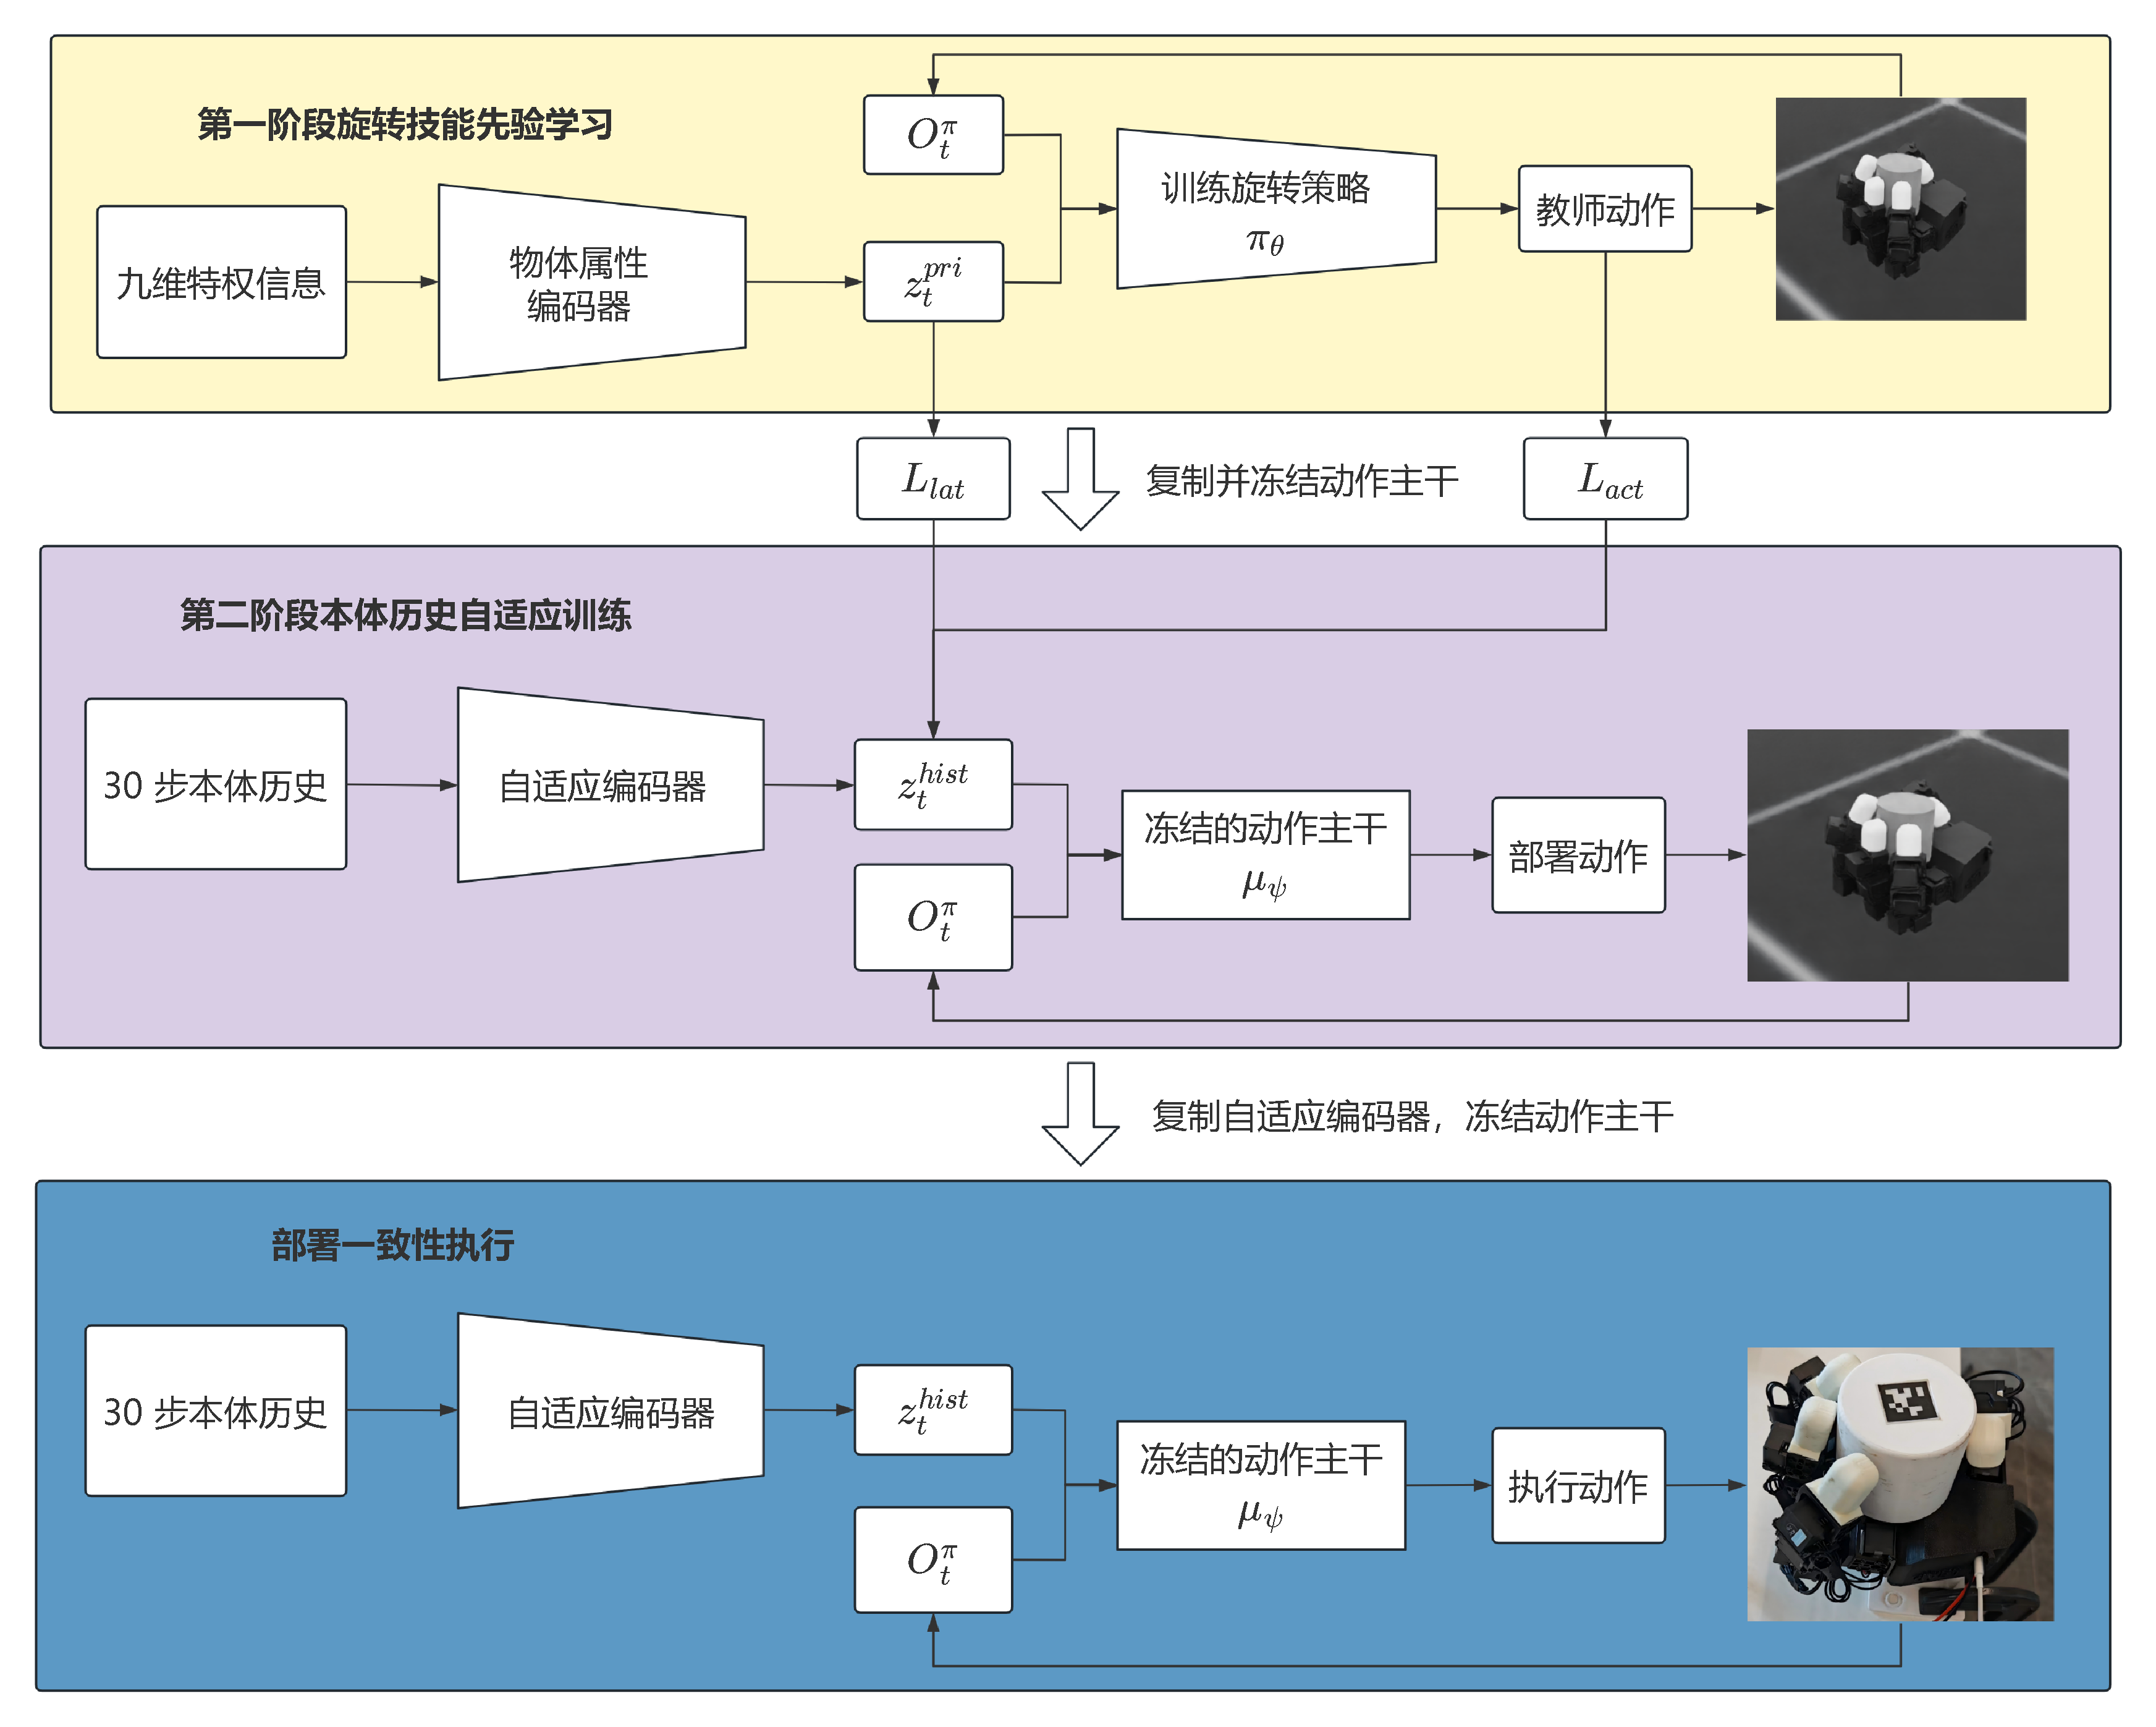
\includegraphics[width=0.90\textwidth]{assets/figures/chapter3/fig3-1_method_framework.pdf}
    \caption{技能先验驱动的两阶段训练与部署执行框架}
    \label{fig:chapter3_framework}
\end{figure}

表 \ref{tab:chapter3_policy_variants} 汇总了本文主要训练与对比的三种策略。三者共享同一动作主干，但输入和训练目标不同：\(\mathrm{Teacher}\) 只在仿真中使用特权信息，是阶段一的参考上界；\(\mathrm{Deploy\text{-}Base}\) 只使用本体历史，不再接触任何对象物理参数，更接近 HORA/RMA 的原始部署思路；\(\mathrm{Deploy\text{-}Refined}\) 则在 \(\mathrm{Deploy\text{-}Base}\) 的基础上加入动作一致性约束，并配合更宽的质心偏移分布，以缓解分布外退化。

\begin{table}[htbp]
    \centering
    \zihao{5}
    \caption{三种策略的输入、训练目标与部署属性}
    \label{tab:chapter3_policy_variants}
    \setlength{\tabcolsep}{3pt}
    \renewcommand{\arraystretch}{1.12}
    \resizebox{\textwidth}{!}{
    \begin{tabular}{p{0.16\textwidth}p{0.15\textwidth}p{0.15\textwidth}p{0.18\textwidth}p{0.20\textwidth}p{0.14\textwidth}}
        \toprule
        策略 & 本体历史 & 特权信息 & 训练目标 & 训练分布 & 可实机部署 \\
        \midrule
        \(\mathrm{Teacher}\) & 短历史观测 & 使用 & PPO 强化学习 & 基础圆柱参数分布 & 否 \\
        \(\mathrm{Deploy\text{-}Base}\) & 使用 & 不使用 & \(L_{\mathrm{lat}}\) & 基础圆柱参数分布 & 是 \\
        \(\mathrm{Deploy\text{-}Refined}\) & 使用 & 不使用 & \(L_{\mathrm{lat}}+\lambda_{\mathrm{act}}L_{\mathrm{act}}\) & 更宽质心偏移分布 & 是 \\
        \bottomrule
    \end{tabular}
    }
\end{table}

从动作接口看，上述三种策略的差别主要在技能先验的来源，而不是控制量的定义。统一写为
\begin{equation}
z_t =
\begin{cases}
z_t^{\mathrm{pri}}=E_{\mathrm{pri}}(\xi_t), & \text{教师侧先验},\\
z_t^{\mathrm{hist}}=E_{\mathrm{hist}}(h_t), & \text{部署侧先验},
\end{cases}
\qquad
\mu_t=\mu_\psi([O_t^\pi;z_t]).
\end{equation}
第一阶段训练时，策略围绕 \(\mu_t\) 构造连续动作分布并采样动作；第二阶段监督和真实部署时，则使用截断后的确定性均值动作。

\subsection{第一阶段：旋转技能先验学习}
\thesisbodyfont
第一阶段的任务是在仿真中先学习稳定的旋转控制能力，获得一个具有较强旋转能力的教师侧控制策略。为此，本文将训练期能够直接读取的对象属性定义为特权信息
\begin{equation}
\xi_t = [p_t^o,\rho,m,\mu,c^\top]^\top \in \mathbb{R}^{9},
\end{equation}
其中 \(p_t^o\) 是物体位置，\(\rho\) 是尺寸参数，\(m\) 是质量，\(\mu\) 是摩擦系数，\(c\) 是质心偏移。随后，特权信息被编码为低维技能先验
\begin{equation}
z_t^{\mathrm{pri}} = E_{\mathrm{pri}}(\xi_t), \qquad z_t^{\mathrm{pri}} \in \mathbb{R}^{8}.
\end{equation}
这里的 \(8\) 维并不是简单压缩，而是刻意把对象属性映射到更贴近控制需求的中间空间：一方面减少策略直接记忆原始物理量的倾向，另一方面也给第二阶段留下一个清晰的监督目标。表 \ref{tab:appendix_direct_priv_ablation} 给出的直接特权输入消融结果进一步说明，原始物理参数直接拼接并没有自动带来更好的教师能力或部署效果，低维技能先验在当前任务中起到了表征约束作用。

将本体观测与技能先验拼接后，第一阶段策略输入写为
\begin{equation}
\bar O_t = [O_t^\pi;z_t^{\mathrm{pri}}].
\end{equation}
在 PPO 训练中，策略网络输出动作分布，价值网络估计回报，策略比率定义为
\begin{equation}
r_t(\theta)=\frac{\pi_\theta(a_t|\bar O_t)}{\pi_{\theta_{\mathrm{old}}}(a_t|\bar O_t)}.
\label{eq:stage1_prob_ratio}
\end{equation}
PPO 的裁剪目标为
\begin{equation}
L_{\mathrm{clip}}(\theta)=
\mathbb{E}_t\!\left[
\min\!\left(
r_t(\theta)\hat A_t,\;
\operatorname{clip}(r_t(\theta),1-\epsilon,1+\epsilon)\hat A_t
\right)
\right],
\label{eq:stage1_ppo_clip}
\end{equation}
其中 \(\epsilon\) 为裁剪系数。综合价值函数损失和熵正则后，第一阶段目标写为
\begin{equation}
\max_{\theta}\;
J_{\mathrm{stage1}}(\theta)
=
L_{\mathrm{clip}}(\theta)
-\lambda_V L_V(\theta)
+\lambda_H H(\pi_\theta),
\label{eq:stage1_objective}
\end{equation}
其中 \(L_V(\theta)\) 为价值函数损失，\(H(\pi_\theta)\) 为策略熵项。

算法 \ref{alg:stage1_prior_learning} 给出了这一阶段的训练流程。实现上，本文把第一阶段分成轨迹采样和小批量 PPO 更新两个层面：外层并行环境负责收集教师侧数据，内层则在固定采样批次上迭代更新特权信息编码器、策略网络和价值网络。这样做的好处是，训练数据和优化目标都围绕同一套技能先验展开，后面第二阶段学习本体历史时就有了明确的参照。

\begin{algorithm}[H]
  \DontPrintSemicolon
  \caption{第一阶段旋转技能先验学习}
  \label{alg:stage1_prior_learning}
  \KwIn{并行环境 \(\mathcal{E}\)，策略观测 \(O_t^\pi\)，特权信息 \(\xi_t\)，奖励 \(r_t\)}
  \KwHyper{采样步长 \(H\)，外层迭代次数 \(K_1\)，PPO 更新轮数 \(M_1\)，小批量大小 \(B_1\)}
  \KwOut{特权信息编码器 \(E_{\mathrm{pri}}\)，策略 \(\pi_\theta\)，价值函数 \(V_\phi\)}
  \KwInit{\(E_{\mathrm{pri}}\)、\(\pi_\theta\)、\(V_\phi\)，并令 \(\pi_{\theta_{\mathrm{old}}}\leftarrow\pi_\theta\)}
  \BlankLine
  \For{\(k=1,\ldots,K_1\)}{
    \(\mathcal{D}\leftarrow\emptyset\)\;
    \For{\(t=0,\ldots,H-1\)}{
      \(z_t^{\mathrm{pri}}\leftarrow E_{\mathrm{pri}}(\xi_t)\)\;
      \(\bar O_t\leftarrow[O_t^\pi;z_t^{\mathrm{pri}}]\)\;
      \(a_t\sim\pi_{\theta_{\mathrm{old}}}(\cdot|\bar O_t)\)，\(p_t^{\mathrm{old}}\leftarrow\pi_{\theta_{\mathrm{old}}}(a_t|\bar O_t)\)\;
      \(v_t\leftarrow V_\phi(\bar O_t)\)\;
      \((r_t,O_{t+1}^\pi,\xi_{t+1})\leftarrow \mathcal{E}(a_t)\)\;
      \(\mathcal{D}\leftarrow\mathcal{D}\cup\{(\bar O_t,a_t,r_t,v_t,p_t^{\mathrm{old}})\}\)\;
    }
    根据 \(\mathcal{D}\) 计算回报 \(\hat G_t\) 与优势 \(\hat A_t\)\;
    \For{\(m=1,\ldots,M_1\)}{
      采样小批量 \(\mathcal{B}\subset\mathcal{D}\)，并用保存的 \(p_t^{\mathrm{old}}\) 计算策略比率\;
      按式 \eqref{eq:stage1_prob_ratio} 和式 \eqref{eq:stage1_objective} 计算 PPO 更新目标\;
      对 \(E_{\mathrm{pri}}\)、\(\pi_\theta\)、\(V_\phi\) 执行 Adam 更新\;
    }
    \(\pi_{\theta_{\mathrm{old}}}\leftarrow\pi_\theta\)\;
  }
  \KwReturn{\(E_{\mathrm{pri}},\pi_\theta,V_\phi\)}
\end{algorithm}

因此，第一阶段得到的是带特权信息的教师侧旋转策略，而不是最终部署策略。它的主要作用是形成稳定动作主干和可监督的技能先验空间，使第二阶段能够在同一动作接口下学习本体历史适应模块。

\subsection{第二阶段：本体历史自适应训练}
\thesisbodyfont
第一阶段用到了特权信息，但这部分信息在真实部署时并不存在。因此，第二阶段必须把“依赖对象参数”的能力，转成“只看本体历史也能估计”的能力。为此，本文冻结第一阶段已经学到的动作主干，仅训练历史编码器 \(E_{\mathrm{hist}}(\cdot)\)，让系统从本体感觉历史中恢复和教师侧一致的技能先验。设第二章定义的本体历史为
\begin{equation}
h_t =
\left[
o_{t-29};o_{t-28};\ldots;o_t
\right]
\in \mathbb{R}^{30\times 32},
\end{equation}
则部署侧技能先验写为
\begin{equation}
z_t^{\mathrm{hist}} = E_{\mathrm{hist}}(h_t), \qquad z_t^{\mathrm{hist}} \in \mathbb{R}^{8}.
\end{equation}

本文采用固定长度的 \(30\) 步本体感觉历史作为适应输入。在约 \(30\,\mathrm{Hz}\) 的控制频率下，该窗口覆盖约 \(1\,\mathrm{s}\) 的近期关节响应，既包含若干次动作更新后的动态线索，又不会使真实部署端缓存过长。表 \ref{tab:appendix_history_length_ablation} 显示，历史长度继续增加并不带来单调收益，因此 \(30\) 帧主要是历史覆盖、旋转效率和部署开销之间的折中。

历史编码器采用一维时序卷积结构。具体而言，单帧 \(32\) 维本体观测先经过两层线性映射和 ReLU 激活得到通道特征，随后沿时间维依次通过三层一维卷积进行聚合，最后展平并投影到 \(8\) 维技能先验空间。相较于直接展平历史窗口，卷积结构能够显式利用相邻时刻的局部变化；与递归结构相比，它在部署端不需要维护额外隐状态。表 \ref{tab:appendix_encoder_structure_ablation} 给出的结构消融也支持这一选择。

第二阶段只训练历史编码器，同时冻结动作主干，原因主要有三点。其一，冻结动作主干可以保留第一阶段已经形成的稳定动作生成方式，降低监督训练破坏原有旋转行为的风险。其二，将适应问题限制在 \(8\) 维技能先验空间内，可以降低从本体历史到动作的学习难度。其三，教师侧和部署侧共享同一动作接口，便于后续直接比较两者的输出差异。

表 \ref{tab:chapter3_policy_variants} 里的 \(\mathrm{Deploy\text{-}Base}\) 可视为更接近 HORA/RMA 原始部署思路的对照基线：它仅通过特征对齐完成从教师侧到部署侧的迁移，不额外引入动作一致性约束或更宽的质心偏移分布。与之相比，\(\mathrm{Deploy\text{-}Refined}\) 在保留这一基本框架的基础上进一步加入动作一致性约束，并配合更宽的质心偏移分布，以减轻 OOD 条件下的性能退化。

第二阶段的教师侧与部署侧动作均由同一冻结后的动作主干产生，分别记为
\begin{equation}
\mu_t^{\mathrm{tea}} =
\mu_\psi\!\left([O_t^\pi;z_t^{\mathrm{pri}}]\right),
\qquad
\mu_t^{\mathrm{dep}} =
\mu_\psi\!\left([O_t^\pi;z_t^{\mathrm{hist}}]\right).
\end{equation}
第一项监督历史编码器恢复技能先验，因此定义潜变量一致性损失
\begin{equation}
L_{\mathrm{lat}}
=
\left\|
z_t^{\mathrm{hist}}-z_t^{\mathrm{pri}}
\right\|_2^2,
\end{equation}
第二项则直接对齐教师和部署动作
\begin{equation}
L_{\mathrm{act}}
=
\left\|
\operatorname{clip}(\mu_t^{\mathrm{dep}},-1,1)
-
\operatorname{clip}(\mu_t^{\mathrm{tea}},-1,1)
\right\|_2^2.
\end{equation}
于是第二阶段总损失为
\begin{equation}
L_{\mathrm{stage2}}
=
L_{\mathrm{lat}}
+\lambda_{\mathrm{act}}L_{\mathrm{act}},
\end{equation}
其中 \(\lambda_{\mathrm{act}}\) 为动作一致性权重。前者保证历史编码器学到的表示和教师侧技能先验保持接近，后者则进一步约束最终动作输出，避免部署侧在未见参数条件下出现明显偏移。

与第一阶段不同，第二阶段的训练数据并不是离线固定数据集，而是由部署侧闭环采样得到。每一步都由策略与环境交互，再用新观测更新历史窗口 \(h_t\)，因此历史编码器实际上是在一个与真实部署更接近的闭环条件下被训练出来的。为了处理 OOD 退化，本文又将对象参数分布扩展为更宽的风险分布 \(p_{\mathrm{risk}}(\eta)\)，使历史编码器在训练时能见到更多质心偏移样本。相应地，基础策略和增强策略在训练分布上的差别写成
\begin{equation}
\eta \sim p_{\mathrm{risk}}(\eta),
\qquad
p_{\mathrm{risk}}(c)\supset p_{\mathrm{base}}(c).
\end{equation}
这一步并不是重新定义任务，而是把第二阶段的适应压力显式推到更容易失真的对象参数上。

算法 \ref{alg:stage2_adaptation_learning} 给出了第二阶段训练流程。冻结动作主干后，训练过程只更新历史编码器，并在每个闭环采样周期中同时计算潜变量一致性和动作一致性两项损失。这样既保留了第一阶段形成的动作模式，也使部署侧输出能够在监督信号下向教师侧动作靠近。

\begin{algorithm}[H]
  \DontPrintSemicolon
  \caption{第二阶段面向风险对齐的本体历史自适应训练}
  \label{alg:stage2_adaptation_learning}
  \KwIn{向量化环境 \(\mathcal{E}\)，策略观测 \(O_t^\pi\)，本体感觉历史 \(h_t\)，特权信息 \(\xi_t\)}
  \KwHyper{对象参数分布 \(p(\eta)\)，更新步数 \(K_2\)，动作一致性权重 \(\lambda_{\mathrm{act}}\)，学习率 \(\beta\)}
  \KwOut{历史编码器 \(E_{\mathrm{hist}}\)}
  \KwFreeze{\(E_{\mathrm{pri}}\) 与 \(\mu_\psi\)}
  \KwInit{\(E_{\mathrm{hist}}\)，Adam 优化器}
  \BlankLine
  采样 \(\eta\sim p(\eta)\) 并重置环境，初始化 \(O_t^\pi\)、\(h_t\) 与 \(\xi_t\)\;
  \For{\(k=1,\ldots,K_2\)}{
    \(z_t^{\mathrm{pri}}\leftarrow E_{\mathrm{pri}}(\xi_t)\)\;
    \(z_t^{\mathrm{hist}}\leftarrow E_{\mathrm{hist}}(h_t)\)\;
    \(\mu_t^{\mathrm{tea}}\leftarrow \mu_\psi([O_t^\pi;z_t^{\mathrm{pri}}])\)\;
    \(\mu_t^{\mathrm{dep}}\leftarrow \mu_\psi([O_t^\pi;z_t^{\mathrm{hist}}])\)\;
    \(\tilde\mu_t^{\mathrm{tea}}\leftarrow \operatorname{clip}(\mu_t^{\mathrm{tea}},-1,1)\)\;
    \(\tilde\mu_t^{\mathrm{dep}}\leftarrow \operatorname{clip}(\mu_t^{\mathrm{dep}},-1,1)\)\;
    \(L_{\mathrm{lat}}\leftarrow \operatorname{mean}\|z_t^{\mathrm{hist}}-z_t^{\mathrm{pri}}\|_2^2\)\;
    \(L_{\mathrm{act}}\leftarrow \operatorname{mean}\|\tilde\mu_t^{\mathrm{dep}}-\tilde\mu_t^{\mathrm{tea}}\|_2^2\)\;
    \(L_{\mathrm{stage2}}\leftarrow L_{\mathrm{lat}}+\lambda_{\mathrm{act}}L_{\mathrm{act}}\)\;
    对 \(E_{\mathrm{hist}}\) 执行 Adam 更新，使 \(L_{\mathrm{stage2}}\) 最小化\;
    执行部署侧动作 \(a_t\leftarrow \tilde\mu_t^{\mathrm{dep}}\)，得到新观测 \(O_{t+1}^\pi\)、\(h_{t+1}\) 与终止标志\;
    若回合结束，则重新采样 \(\eta\sim p(\eta)\) 并重置环境\;
  }
  \KwReturn{\(E_{\mathrm{hist}}\)}
\end{algorithm}

\subsection{部署执行阶段}
\thesisbodyfont
部署阶段不再做策略训练，而是把第二阶段得到的历史编码器直接用于仿真评测和真实 LEAP Hand 部署。系统在这一阶段只保留真实平台可直接读取的本体感觉观测 \(O_t^\pi\) 和历史窗口 \(h_t\)，再由历史编码器估计技能先验并输出动作：
\begin{equation}
a_t^{\mathrm{dep}}
=
\operatorname{clip}\!\left(
\mu_\psi\!\left([O_t^\pi;E_{\mathrm{hist}}(h_t)]\right),
-1,1
\right).
\end{equation}
随后动作通过第二章定义的关节目标更新方式送入底层位置控制器。

真实部署时，系统先执行短时 warmup，缓慢靠近初始抓取姿态，再用当前关节位置和关节目标构造历史窗口。随后控制环以 \(30\,\mathrm{Hz}\) 运行，历史编码器连续更新，策略每一步输出相对关节目标增量，由底层控制器完成具体驱动。为降低启动冲击，本文在初始抓取阶段保留较小闭合系数，并采用保守的电机增益设置；这一设置优先保证真实平台闭环稳定，再讨论旋转效率。

从控制意义上看，部署阶段本质上是把第二阶段学到的历史适应能力转成真实系统上的连续控制能力。只要历史编码器能稳定恢复技能先验，部署策略就可以在不依赖对象质量、摩擦和质心参数的条件下完成动作推理。这也是本文在第四章中能够直接用同一策略做仿真评测和实机验证的原因。

\subsection{本章小结}
\thesisbodyfont
本章提出了技能先验驱动的两阶段本体自适应旋转框架。第一阶段利用仿真中的特权信息学习旋转技能先验和教师策略，第二阶段冻结动作主干，只训练历史编码器从本体感觉历史中恢复同一技能先验，并通过动作一致性约束和更宽的风险参数分布提升部署侧鲁棒性。最后，本文给出了部署执行阶段的控制方式，使仿真训练、统一评测和真实部署共享同一动作接口。该框架为第四章的仿真评测和实机验证提供了直接的方法基础。
